\section{\system Design}
\label{sec:system}
We now provide an overview of \system and it's architecture and discuss how it evolved via participatory design. 

%the key components that provide the foundation for \system, which instruments the design goals outlined in Section~\ref{sec:design_goal}. 
%We then explain the system architecture of \system.

\subsection{Participatory Design}

Inspired by earlier work~\cite{bauerle2022symphony, rahman2020mixtape}, we conducted several participatory design sessions after developing the initial \system framework. These sessions aimed to understand the specific needs of data science workers and then design and develop a core set of \system components and widgets. We conducted weekly sessions over a six-week period focusing on three different projects related to knowledge acquistion and integration. These projects involved several collaborators in various roles within \company 
from researchers ($N=6$) %meg meetings: Estevam, Nikita, Nedelina, Hannah, Sajjadur, Tom 
and engineers ($N=4$) % Aiden, Chen, Austin, Dan
to product managers ($N=1$) % James 
and taxonomy architects ($N=4$). % Estevam, Eser, Aiden, Chen
Note that the taxonomy architect role was shared by a subset of 
researchers and engineers within the platform team.
The sessions lasted between 30 minutes and an hour.
The first session with each team involved introducing the core features of \system and the base components. We then asked participants to describe their tasks step by step.
While the weekly sessions involved the entire platform team, 
we also arranged ad-hoc participatory sessions
with individual project leaders for a deeper dive into 
the project-specific requirements and 
iteratively refined \system features.

% \begin{figure}[!htb] 
%   \centering %trim=left bottom right top
%   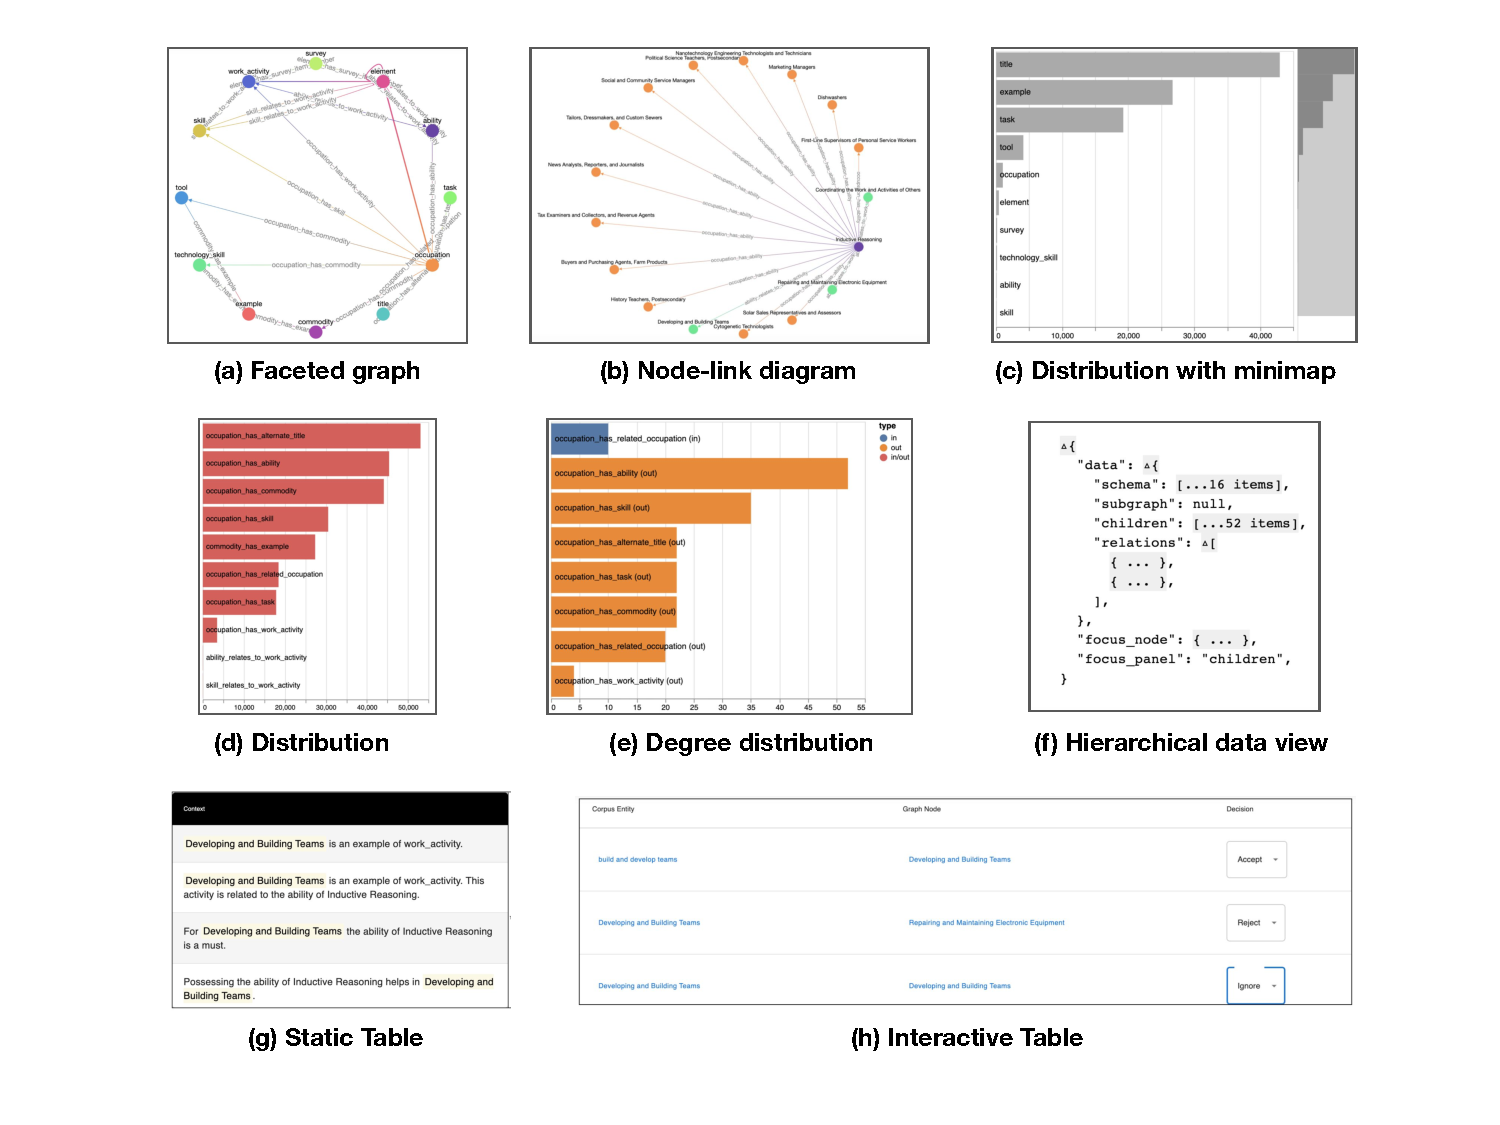
\includegraphics[width=0.8\linewidth,trim={50 35 40 15},clip]{figures/components.pdf}
%   \caption{\system base components: (a) faceted graph, (b) node-link diagram, (c) distributions with minimap, (d) distributions, (e) relation degree distributions, (f) hierarchical data viewer, (g) static table, and (h) interactive table.}
%   \label{fig:defaults} 
% \end{figure}

\begin{figure*}[!htb] 
  \centering
  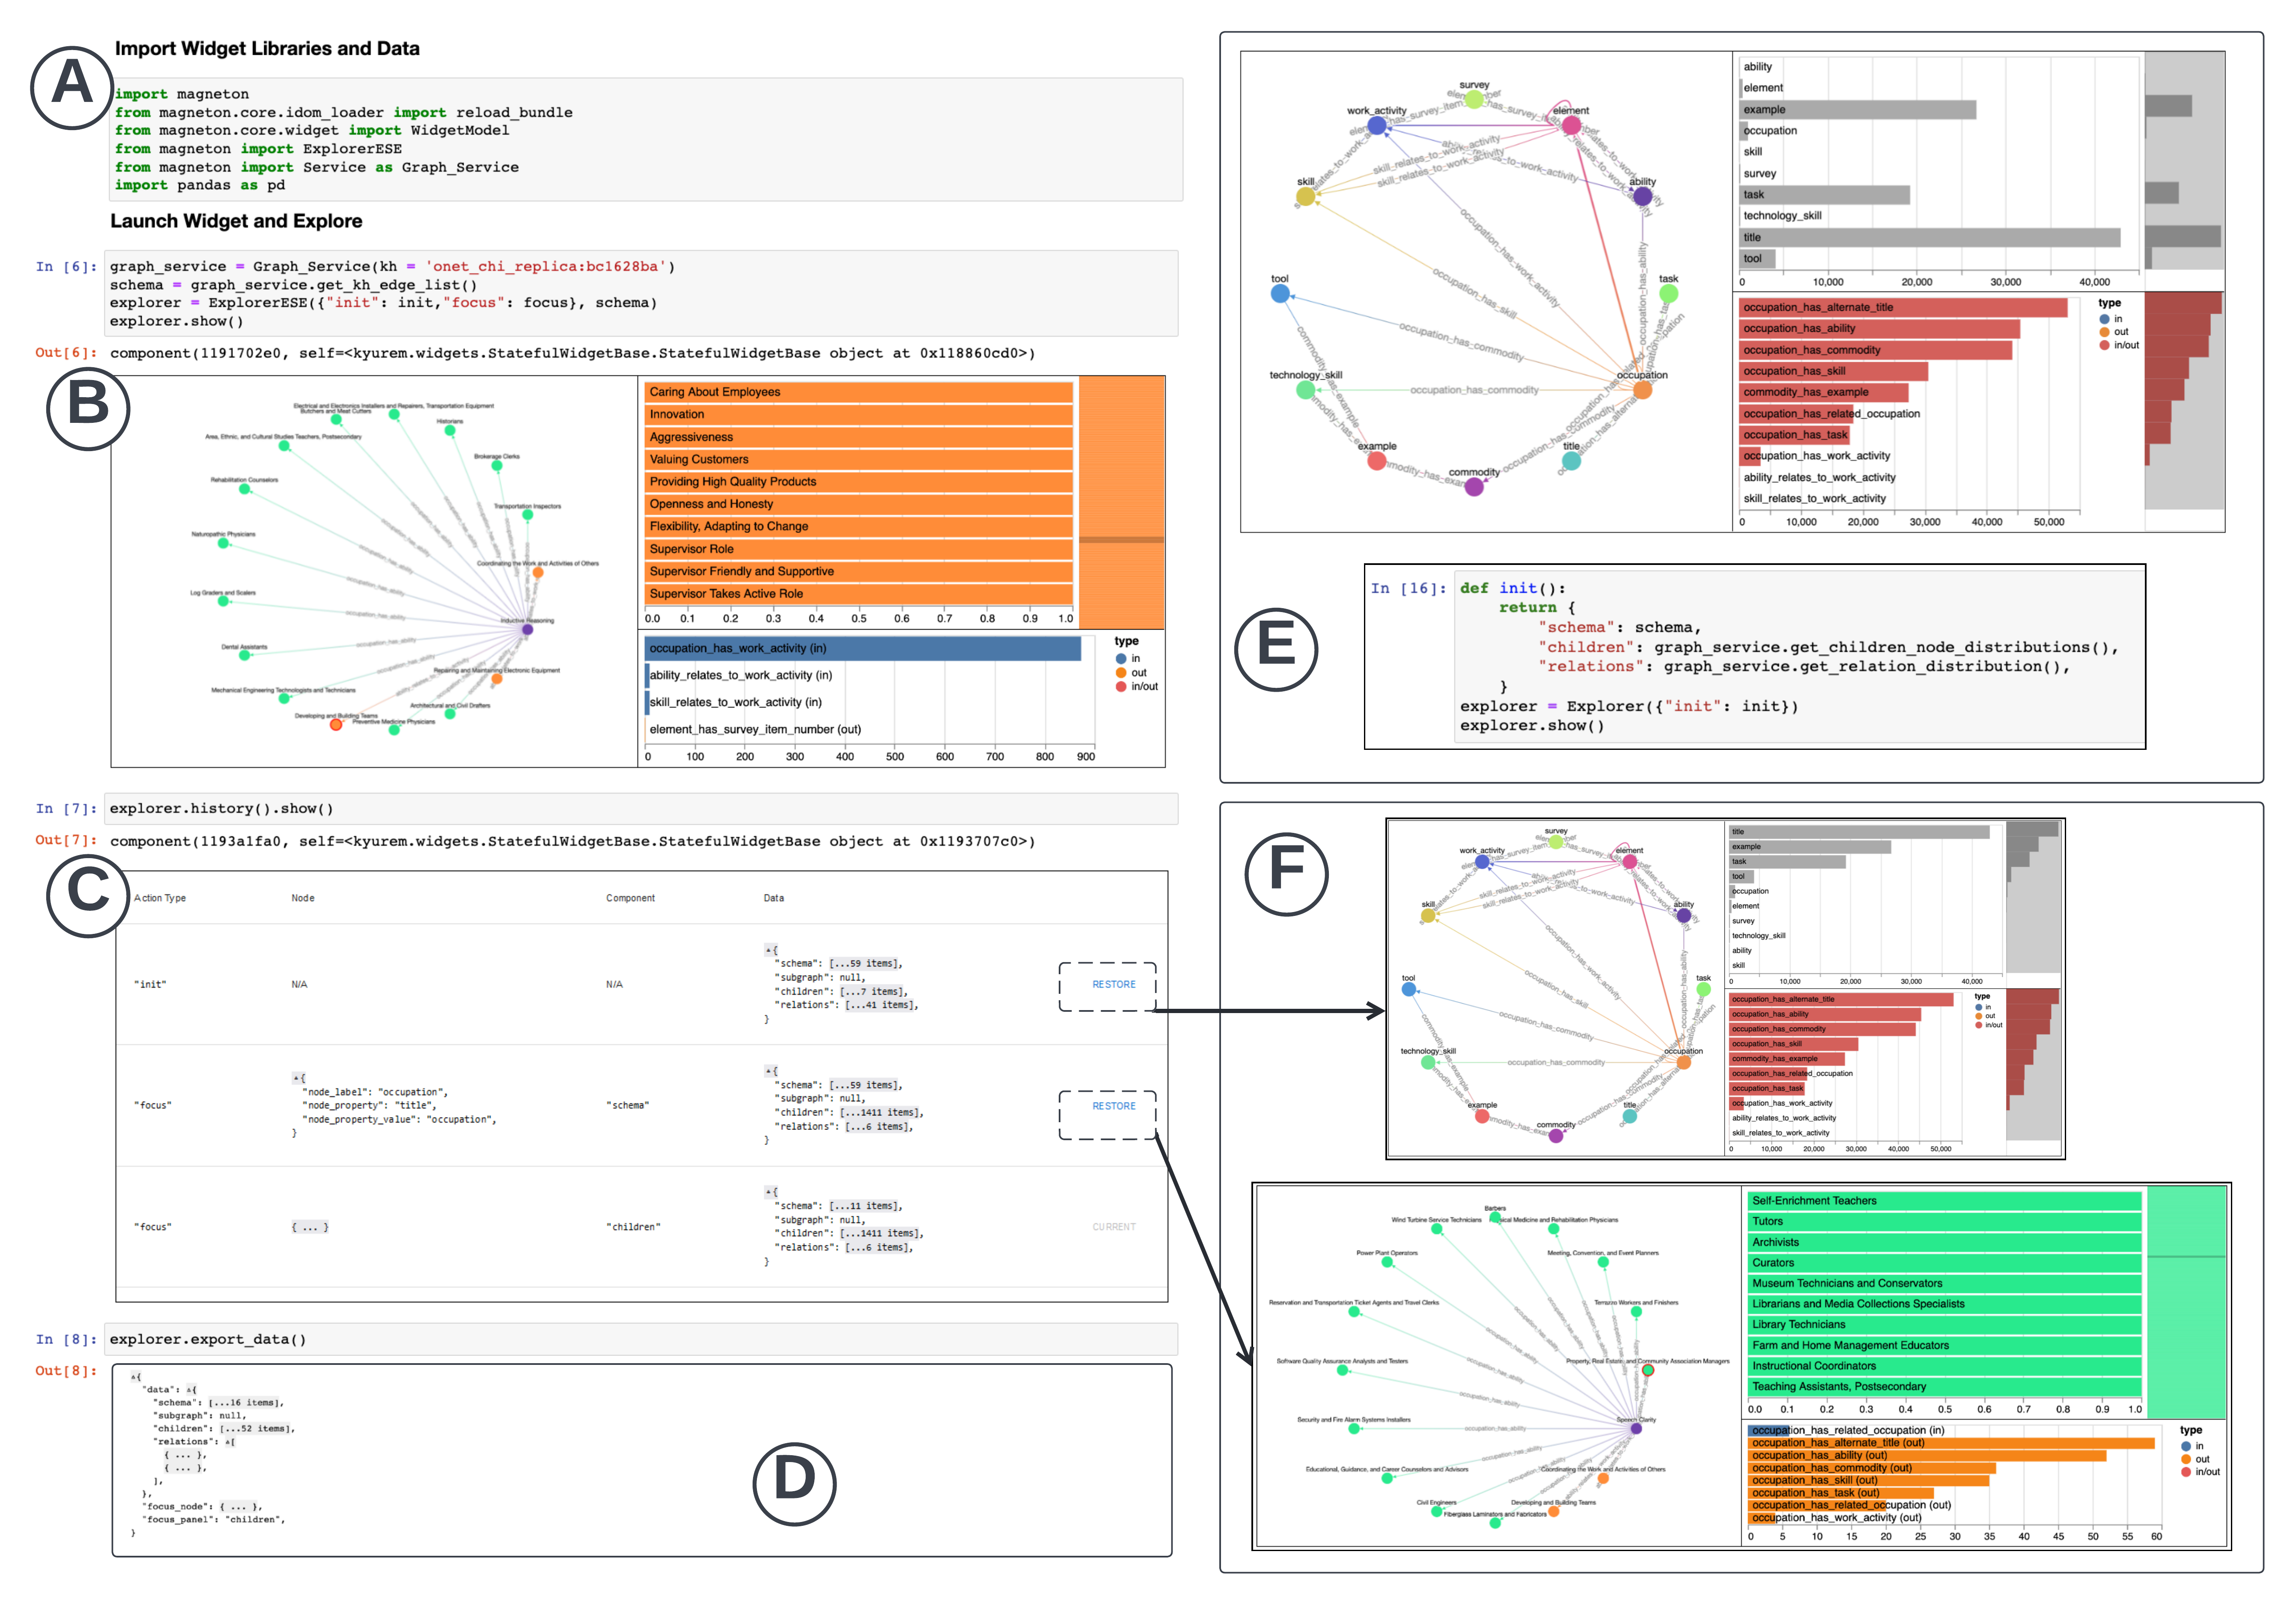
\includegraphics[width=\linewidth]{figures/teasernew.png}
  \caption{Screenshot of a knowledge acquisition workflow using \system widget library. (a, b) importing libraries to launch a multiple-coordinated view widget, (c) leveraging the history view of \basesystem to context switch between exploration history, (d, e, f) viewing and exploring multi-modal data interactively and programmaticially.}
  \label{fig:alignment-verification} 
\end{figure*}

We collected several systems- and feature-level enhancement requests for \system from these participatory design sessions. These requests fall into three themes: data modality (\ie ability to explore multi-modal data such as text, JSON documents, and graphs), perceptual scalability (\ie ease of overviewing large-scale data), and synchrony of navigation (\ie seamless context switching among multiple-coordinated views.) Based on the participant feedback, we implemented eight basic components shown in Figure~\ref{fig:defaults} in Appendix~\ref{app_sec:components}. These components were designed to support various enhancements and augmentation requests 
mentioned above: multi-modal data exploration (components b,f,g, and h in Figure~\ref{fig:defaults}),
(ii) scalable overview via faceted graph (component a in Figure~\ref{fig:defaults}), and (iii) multiple-coordinated views achieved by combining components into widgets (Figure~\ref{fig:ese-explorer}.)
We provide a detailed account of how the participatory session with participants helped prioritize the select of these components in Appendix~\ref{app_sec:components}. 

\subsection{\system System Architecture}
Figure~\ref{fig:archi} provides an overview of the system we developed to support graph exploration and analysis using the \system library. At the heart of the system is the \system widget suite, a collection of widgets that support programmatic and interactive graph exploration within computational notebooks. The base widget in the suite is extended from the \basesystem framework~\cite{choi2023towards}. Users' actions in the front-end components trigger various functions, via Graph Service, in the back-end.
% \begin{figure}[!htb] 
%   \centering
%   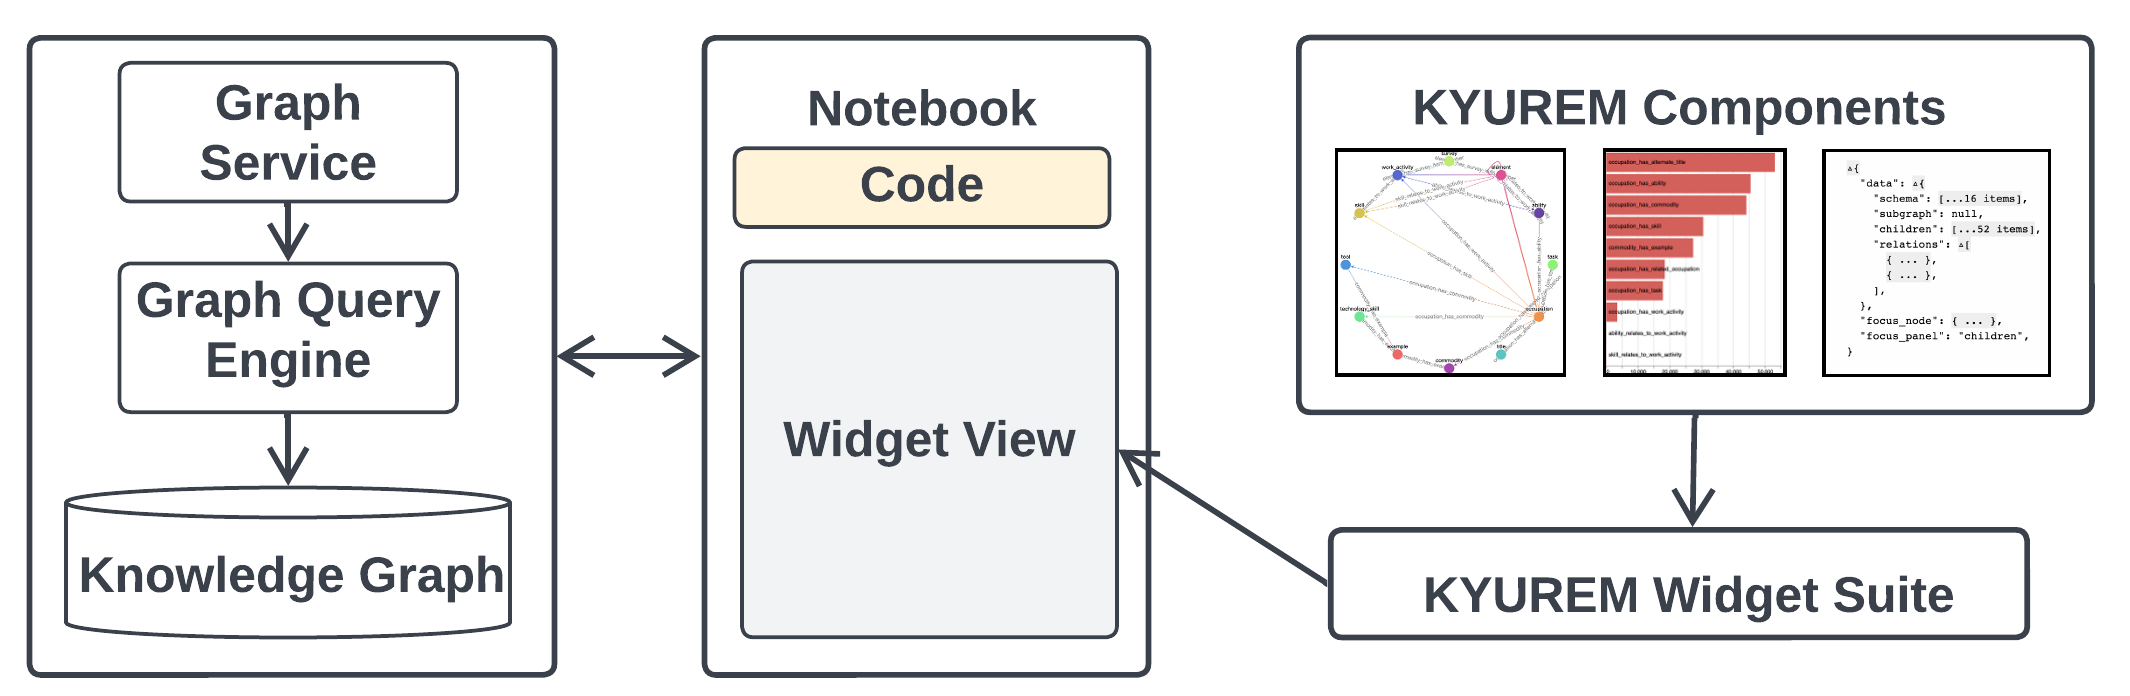
\includegraphics[width=0.5\linewidth]{figures/kyurem-archi.png}
%   \caption{System architecture for graph exploration with \system widget suite.}
%   \label{fig:archi} 
%   \Description{System Architecture.}
% \end{figure}
Examples of graph-specific operations include generating graph schema, finding node neighborhoods, and computing distributions of nodes and relations, among others. The operations are part of an in-house graph query library, which is published as a Python package. Each operation is mapped to the corresponding graph query, which is executed by the graph query manager and returned to the front-end. Note that the graph data operations can be initiated from the widget, notebook, or the front-end components. 

% Users can access the current data state of the widget using data accessor functions that return JSON objects. Note that another class of action, called transient action, does not update the data state. Examples include selection events triggered by simultaneous clicking of the mouse and ``CTRL'' button. We do not display the transient actions in the interaction history. However, we discuss later how we implemented custom accessor functions to access these states (see Listing~\ref{list:export}.) The update of the data state in the widget model triggers a re-render of the front-end component, which is contained in the widget view. We further augmented the widget view design to enable robust synchronization between the widget model and view, which we discuss next.

% \begin{listing}[!htb]
% \begin{minted}
% [
% framesep=2mm,
% baselinestretch=0.6,
% fontsize=\footnotesize
% ]
% {python}
% # Import widget and graph API libraries
% from magneton import Explorer
% from magneton import Graph_Service as gs

% # Connect to Graph
% graph = gs(server_url)

% # Load graph schema in a variable
% schema = gs.get_schema()

% # Load and display widget
% explorer = Explorer(schema)
% explorer.show()

% # Load and view interaction history
% provenance = explorer.history()
% provenance.show()
% \end{minted}
% \caption{Load widget and view provenance.}
% \label{list:export}
% \end{listing}

% \subsubsection{Customizable and transparent actions}
% The ipywidgets model and view synchronization is managed by, \emph{Comm}, a communication API. 
% However, to enable interaction-aware updates in the widget model and triggering of appropriate data operations corresponding to an event in the front-end component, we implement an action wrapper (see Figure~\ref{fig:stateful_widget}.) 
% The action wrapper packages and dispatches an action --- consisting of information such event type, item, and component where event occurred --- via the communication API. Each component may contain one or more event listeners corresponding to specific event, \ie user interaction such as select, group, filter. 
% Each event listener corresponds to a data operation. 
% \system's events were derived from common interactions found in graph task taxonomies~\cite{pretorius2014tasks, kerracher2015task, ahn2013task, lee2006task}, surveys~\cite{liu2018graph, 2019_eurovis_mvnv, pienta2015scalable}, exploratory data analysis literature~\cite{yi2007toward, amar2005low}, and then refined further based on the participant requests during the contextual inquiry study.

% \begin{listing}[!htb]
% \begin{minted}
% [
% framesep=2mm,
% baselinestretch=0.6,
% fontsize=\footnotesize
% ]
% {python}
% # Get current state data
% explorer.export_data()

% # Get list of transient selections
% explorer.export_selection(sync=False)
% \end{minted}
% \caption{Export data and transient selection.}
% \label{list:load}
% \end{listing}

% Within the stateful widget, the reducer updates the data state according to the executed data operation.
% \system enables customization of these data operations from the notebook. For example, a developer may define data operation to return a distribution sorted by descending order of node frequency. However, the user may prefer viewing the distribution in alphabetic order. 
% Unfortunately, current solutions such as Symphony~\cite{bauerle2022symphony} lack the affordances for such customization.
% In the absence of an explicit \emph{sort order} parameter, the user has to request the widget developer to add or update the data operation manually. Furthermore, the developer has to update and release a new Python package before the feature becomes available, which is a cumbersome experience. To address this limitation, \system 
% introduces a special action class called \emph{shared actions}.
% Shared actions are mapped to functions defined by the user in
% the notebook. 
% When a shared action is triggered via user interaction on the
% front-end component, \system leverages the action wrapper in the widget view and the reducer in the widget
% to execute the corresponding user-defined function 
% and synchronize the widget model and front-end component state. 
% Listing~\ref{list:shared} shows an extreme
% example of shared action where even the initial rendering of the widget is user-defined.
% The corresponding front-end view for the widget is 
% shown in Figure~\ref{fig:explorer_widget}.

% \begin{listing}[!htb]
% \begin{minted}
% [
% framesep=2mm,
% baselinestretch=0.6,
% fontsize=\footnotesize
% ]
% {python}
% # User defined function generating schema
% # node and relation distributions
% # for corresponding front-end components
% def init_full():
%     return {
%         "schema": gs.get_schema(),
%         "node": gs.get_node_distribution(),
%         "relation": gs.get_relation_distribution()
%     }
    
% # Initialize widget with the callback function
% explorer = Explorer({"init":init_full})
% explorer.show()
% \end{minted}
% \caption{Customize data operation.}
% \label{list:shared}
% \end{listing}

% The capability to share functions enables greater customization as users can keep updating the shared action outcomes to explore different
% objectives by modifying the function defined in the notebook. 
% For the widget initialization example discussed earlier,
% participants may change the schema computation function 
% to obtain the schema of a specific sub-graph. User may add
% wrapper functions on top of the distribution computation functions
% to reorder the distributions.
% However, the output of the wrapper has to be consistent with the expected data format for the front-end component. 
% The stateful widget propagates exceptions to the front-end to ensure transparent communication of any such inconsistency. Such transparency enables the user to debug while writing custom shared functions in the notebook.
% The shared actions also allow for \emph{DRY} (Don't Repeat Yourself)~\cite{foote2014learning} programming practices, as one function definition can be used by 
% both the front-end component and the stateful widget model. However, user-defined customizations may apply to 
% only the actions declared as shared.
% Moreover, in the current version of \system, only actions
% declared within the widget model as shared can be customized.



%\hkc{describe the system v0 that was used in this session. e.g., The design session was conducted using an initial version of our system that contain xxx,yyy, components.}

% \todo{basic: Pane, faceted graph, distribution, provenance json, persistent selection}

% \todo{requested: sub-graph, mini-map, degree, hierarchal data view, static, and interactive tables, tabular provenance, transient selection, geometric zooming and node-link diagram adjustment.}








